\documentclass[sigconf]{acmart}

\settopmatter{printacmref=false} % Removes citation information below abstract
\renewcommand\footnotetextcopyrightpermission[1]{} % removes footnote with conference information in first column
\pagestyle{plain} % removes running headers

\usepackage[utf8]{inputenc}	
\usepackage[T1]{fontenc}

\usepackage{multirow}
\usepackage{booktabs} 
\usepackage{colortbl}
\usepackage{todonotes}
\usepackage{algorithm}
\usepackage{algorithmic}
\usepackage{pdfpages}
\usepackage{balance}
\usepackage{mdframed}
\usepackage{hyperref}

\usepackage[labelformat=simple]{subcaption}
\renewcommand\thesubfigure{(\alph{subfigure})}
\definecolor{Gray}{gray}{0.9}
 
\setcopyright{rightsretained}

\begin{document}
	
\title{Airbnb - New York’s Analysis}

\author{Jackson A. Prado Lima}
\affiliation{
	\institution{Department of Computer Science, Federal University of Paran\'{a}}
	\city{ CP:19081, CEP: 81531-980, Curitiba} 
	\state{Paran\'{a}}
	\country{Brazil}
}
\email{japlima@inf.ufpr.br} 
	
\renewcommand{\shortauthors}{J. A. Prado Lima}
\renewcommand{\shorttitle}{Airbnb - New York’s Analysis}

\begin{abstract}
	Airbnb is an outstanding hosting service used worldwide and provides information to its users in a simple and efficient manner, although this information is limited only to listings of its products. In this work, an analysis is made taking into account if incidents and cultural organizations influence the prices practiced in Airbnb. Besides, the prediction of new prices is carried out that the user can come to inform taking into account information of the current listings. The price forecast has some advantages when advising the user: on the price practiced (is too large or small), the mode of advertisement, or even on the investment decisions of the market analysis. To help in this task, the present work performs an analysis using graphs, maps and different types of machine learning. The data reveals that Queens district has the more adequate trade-off among price, cultural organization, and incidents as well as the accommodates diversity. Besides, cultural organization has a high influence in to predict price.
\end{abstract}

%\keywords{BigData, Machine Learning, Airbnb} 

\maketitle

%%%%%%%%%%%%%%%%%%%%%%%%%%%%%%%%%%%%%%%%%%%%%%%%%%%%%%%%%%%%%%%%%%%%%%%%%%%%%%%%%%%%%%%%%%%%%%%%%%%%%%%%%%%%%%%%%%%%%%%%%%%
%\vspace{-0.2cm}
\section{Introduction}

Airbnb was founded in August of 2008 and based in San Francisco, California. Airbnb is an online marketplace and hospitality service, enabling people to lease or rent short-term lodging including vacation rentals, apartment rentals, homestays, hostel beds, or hotel rooms. 

%The company does not own any lodging; it is merely a broker and receives percentage service fees (commissions) from both guests and hosts in conjunction with every booking. It has over 3,000,000 lodging listings in 65,000 cities and 191 countries, and the host sets the cost of accommodation. Like all hospitality services, Airbnb is a form of collaborative consumption and sharing. Airbnb has two million rooms available - nearly three times more than that of the largest hotel chain in the world. 

Airbnb has help a lot of people, but how can we predict a price or if the cultural organizations and incidents impacts on listing price? In some moments, the guests want to a local cheap or more attractive considering local events to appreciate. Thus, predicting a cheap and safe local is arguably important. In this paper, we try and capture this characteristic using maps, charts and machine learning to help the guest in the chose.

The paper is organized as follows. Section~\ref{sec:experiment_description} describes how the experimental evaluation was conducted. Section~\ref{sec:results} presents and analyses the results obtained. Finally, Section~\ref{sec:conclusion} concludes the paper and discusses the future work.

%\vspace{-0.2cm}
\section{Experiment Description}
\label{sec:experiment_description}

The hypothesis of this work\footnote{The project is available at https://github.com/jacksonpradolima/airbnb-ny-analysis} is that our approach is capable to recommend a cheap and safe local (district/borough) as well as consider the influence of these aspect in to predict listing price. To evaluate this, we consider uses maps, charts and machine learning.

According to our goals the experiment was guided by the following researches questions: \textbf{RQ1:} ``How the incidents and cultural organizations impact on listing price?'' and \textbf{RQ2:} ``How the incidents and cultural organizations impact on regression model to predict the listing price?''.

To answer the RQ1 we compared the result shows on maps, a collinearity matrix among the features, and how the accommodates are distributed. To answer the RQ2 we used a machine learning with 7 regression models and the results were compared using Median Absolute Error.

%\vspace{-0.2cm}
\subsection{Target Data}
\label{sec:experiment_description:target_data}

The investigation focused on four dataset collected in open data sites. These dataset are as follows: 1) Listings, a dataset that is a Airbnb snapshot of 02 April, 2017; 2) Incidents, contains all incidents from New York for the year 2016; 3) Cultural Organizations, contains all cultural organizations from New York in 2017; and 4) NYC Borough, contains informations about boundaries of boroughs (districts). Further information about these datasets are available in the Table~\ref{tab:datasets}.

%\vspace{-0.2cm}
\begin{table}[!htpb]
	\fontsize{7pt}{7pt}\selectfont
	\centering
	\caption{Data sets used in the experiment.}
	\label{tab:datasets}
	\begin{tabular}{cp{3.5cm}cc}
		\toprule
		         \textbf{Dataset}          & \textbf{Description}                                                                                                                          & \textbf{Size} & \textbf{Download} \\ \midrule
		   Listings~\cite{base:airbnb}     & Detailed listings data, including various attributes (features) of each listing such as number of bedrooms, bathrooms, location, etc.         &    153,7MB    &        csv        \\ \midrule
		 Incidents~\cite{base:incidents}   & All valid felony, misdemeanor, and violation crimes reported to the New York City Police Department (NYPD) for all complete quarters in 2016. &    124,2MB    &        csv        \\ \midrule
		Cultural Org.~\cite{base:cultural} & Listing of all Cultural Organizations in the Department of Cultural Affairs directory.                                                        &    333,3kB    &        csv        \\ \midrule
		 NYC Borough~\cite{base:borough}   & Polygon boundaries of boroughs (water areas excluded).                                                                                        &    400,5kB    &      GeoJson      \\ \bottomrule
	\end{tabular}
\end{table}

%\vspace{-0.2cm}
%\subsection{Integration Data}
%
%To help in the analyses, the Cultural Organizations and Incidents dataset received a score. How we have 5 districts in New York, and to be easy, the Cultural Organizations and Incidents dataset were grouped and ranked in relation to the order (0-4), where 0 is the worst and 4 the best. In this case, the datasets were ordered by the number in each district, ascendant for Cultural Organizations and descendant for the Incidents. In the end, it was create a unique data frame with the necessary informations that contains 37043 rows. 

\section{Results and Analysis}
\label{sec:results}

This section shows and discusses the results in order to answer the researches questions.

\subsection{Answering RQ1}

Figure~\ref{fig:pairwiserelationsprincipalfeatures} shows, per district, a matrix of each feature as a function of another which is useful to check for any collinearity among the feature. The cells running through the diagonal of the matrix contain a histogram with its values on the X axis. The features chose to be analyzed were: price, cultural organizations and incidents.

\begin{figure}[!htpb]
	\centering
	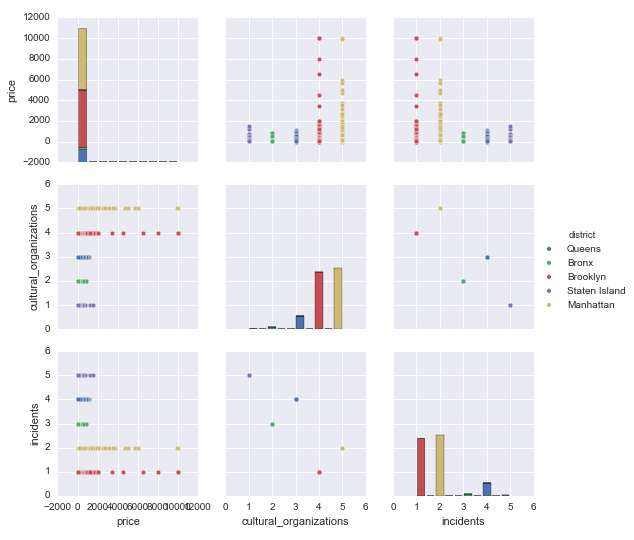
\includegraphics[width=\linewidth]{images/related_data2}
	\caption{}
	\label{fig:pairwiserelationsprincipalfeatures}
\end{figure}

%J: Old
%Based on the figure, we do see that the results are loosely related and not resemblance of a straight line. Thus, there is no strong evidence of collinearity among the features. However, we can observe that Queens and Bronx are in the trade-off among the features. To help in to check this observation, Figure~\ref{fig:datadistribution} shows the data distribution in relation the listings mean price per district (Figure~\ref{fig:datadistribution:price}), the number of cultural organizations per district (Figure~\ref{fig:datadistribution:cultural}), and the number of incidents per district (Figure~\ref{fig:datadistribution:incidents}). We can observe in Figure~\ref{fig:datadistribution:price} that Manhattan district has the highest listings mean price, and Queens and Bronx are the lowest. In Figure~\ref{fig:datadistribution:cultural}, we can observe that Manhattan stands out followed by Brooklyn. On the other hand, Brooklyn stands out followed by Manhattan when we considers incidents (Figure~\ref{fig:datadistribution:incidents}). In this sense, we can to affirm that Queens and Bronx have the best trade-off among mean price, cultural organizations and incidents.

%J: Old
%Based on the figure, we do see that the results are loosely related and not resemblance of a straight line. Thus, there is no strong evidence of collinearity among the features. However, we can observe that Queens and Bronx are in the trade-off among the features. To help in to check this observation, Figure~\ref{fig:datadistribution:price} shows that Manhattan district has the highest listings mean price, and Queens and Bronx are the lowest. In Figure~\ref{fig:datadistribution:cultural}, we can observe that Manhattan stands out followed by Brooklyn. On the other hand, Brooklyn stands out followed by Manhattan when we considers incidents (Figure~\ref{fig:datadistribution:incidents}). In this sense, we can to affirm that Queens and Bronx have the best trade-off among mean price, cultural organizations and incidents.

Based on the figure, we do see that Queens and Bronx are in the trade-off among the features. To help in to check this observation, Figure~\ref{fig:datadistribution:price} shows that Manhattan district has the highest listings mean price, and Queens and Bronx are the lowest. In Figure~\ref{fig:datadistribution:cultural}, we can observe that Manhattan stands out followed by Brooklyn. On the other hand, Brooklyn stands out followed by Manhattan when we considers incidents (Figure~\ref{fig:datadistribution:incidents}). In this sense, we can to affirm that Queens and Bronx have the best trade-off among mean price, cultural organizations and incidents.


\begin{figure}[!htpb]
	\centering
	\begin{subfigure}{0.5\textwidth}
		\centering
		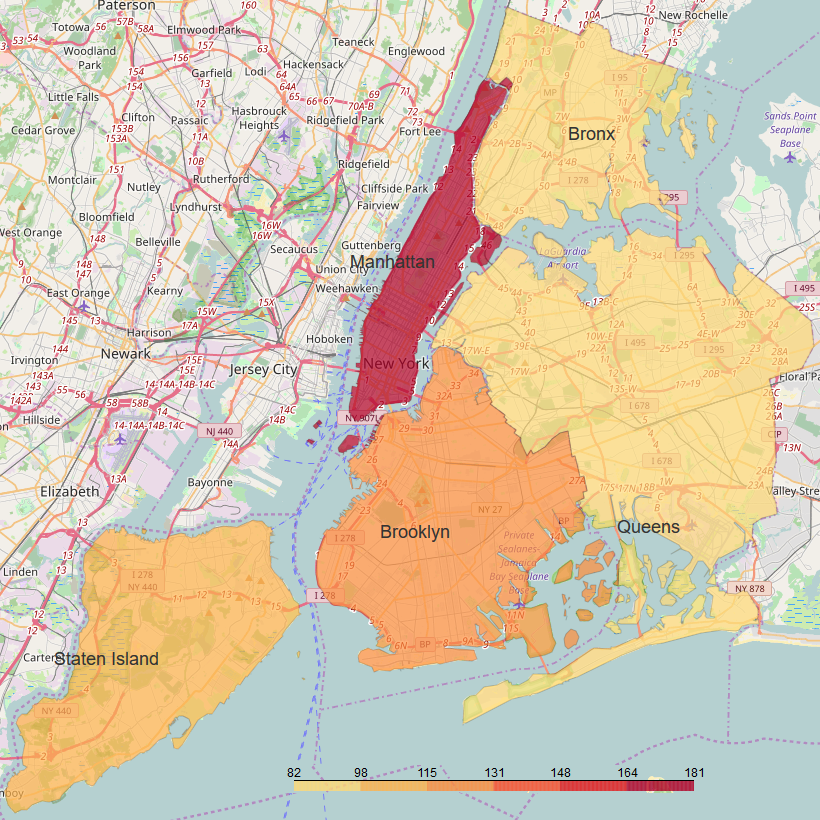
\includegraphics[scale=0.27]{images/price_per_district}
		\caption{Mean Price per District}
		\label{fig:datadistribution:price}
	\end{subfigure}
	\hfill	
	\begin{subfigure}{0.5\textwidth}
		\centering
		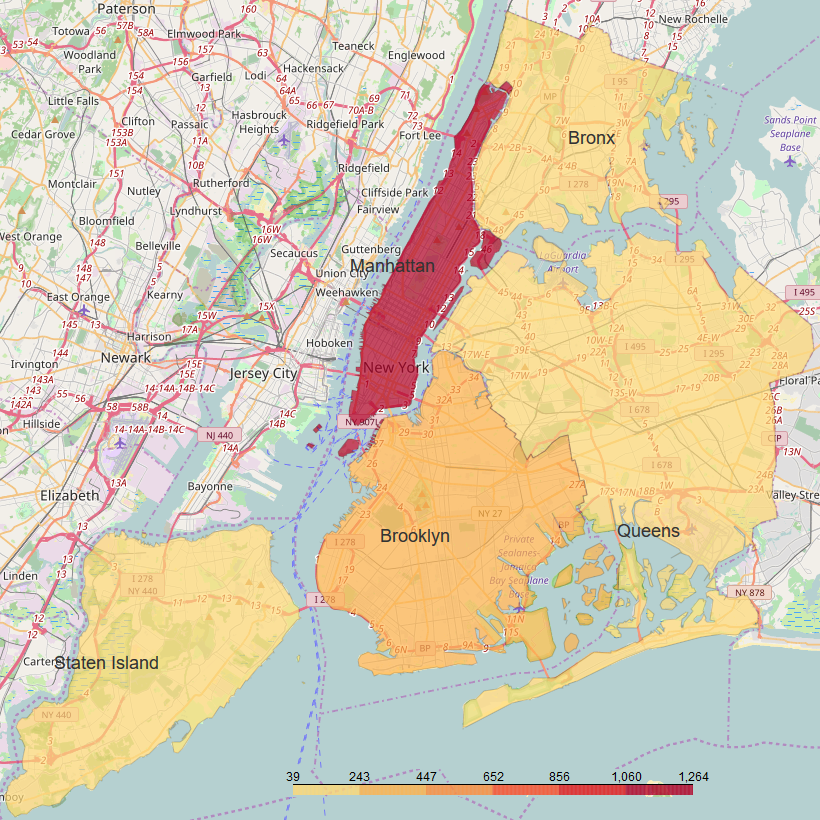
\includegraphics[scale=0.27]{images/cultural_organizations_per_district}
		\caption{N. Cultural Organizations per District}
		\label{fig:datadistribution:cultural}
	\end{subfigure}
	\hfill
	\begin{subfigure}{0.5\textwidth}
		\centering
		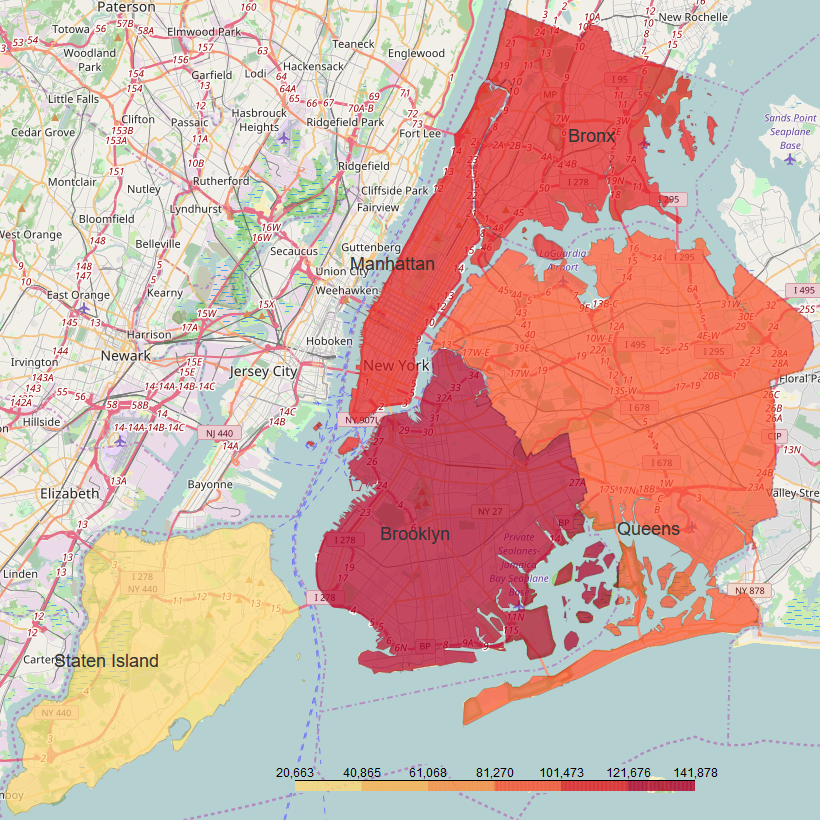
\includegraphics[scale=0.27]{images/incidents_per_district}
		\caption{N. Incidents per District}
		\label{fig:datadistribution:incidents}
	\end{subfigure}
	
	\caption{Data Distribution per District}	
	\label{fig:datadistribution}
\end{figure}

Figure~\ref{fig:meanpriceperaccomodate} shows mean price grouped by the number of people that can accommodate per district: Queens, Manhattan, Bronx, Brooklyn, and Staten Island. We can observe that Manhattan's district has more options than other ones. It's interesting highlight Queens district outperformed Bronx in the diversity of accommodates. 

\begin{figure}[!htpb]
	\centering
	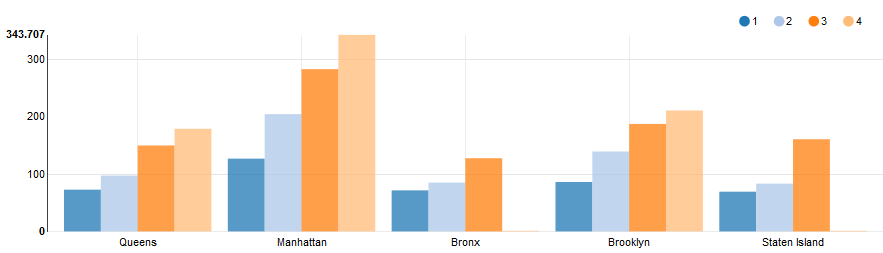
\includegraphics[width=\linewidth]{images/mean_price_per_accomodate}
	\caption{}
	\label{fig:meanpriceperaccomodate}
\end{figure}

Analyzing the results, we can conclude that where it has more cultural organizations is more expensive and consequently attracts more incidents. However, we found two districts in the trade-off among price, cultural organizations and incidents: Queens and Bronx; where comparing these districts Queens outperforms Bronx in the diversity of accommodates.

\subsection{Answering RQ2}

For this analysis using machine learning we split our dataset into a train and test (80/20). We run 7 regression models to calculate the Train and Test Score: Linear Regression, Ridge Regression, Lasso Regression, Elastic Net, Bayes Ridge Regression, Orthogonal Matching Pursuit (OMP), and Gradient Boosting Regressor (GBR). In the analysis, we used 6 regression models and compared with GBR using an exhaustive "grid search" which simply tries all the supplied parameter combinations and uses cross-validation folding to find the best one.

Figure~\ref{fig:medianabsoluteerrorprice} shows the Linear Regression, Ridge Regression, Lasso Regression, Elastic Net, Bayes Ridge Regression, OMP and their Median Absolute Error. Intuitively, Median Absolute Error is less sensitive to outliers than Mean Squared Error and translates nicely to a dollar amount that is relative to price.

\begin{figure}[!htpb]
	\centering
	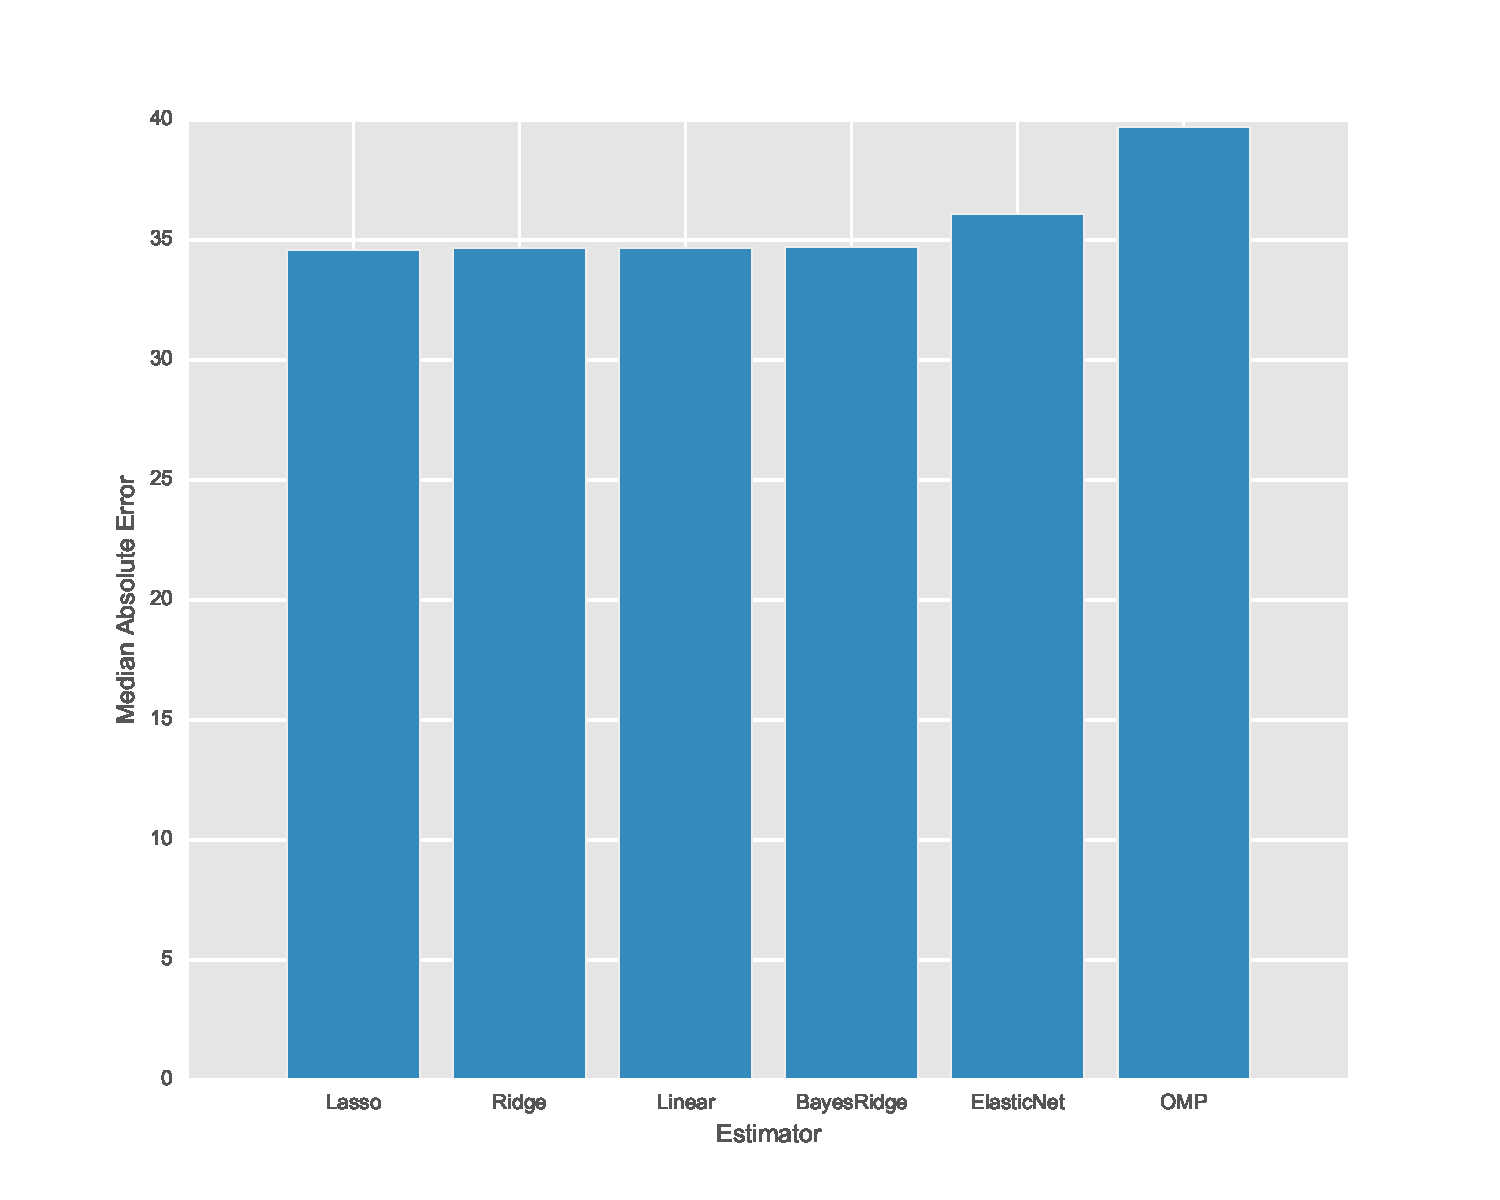
\includegraphics[width=\linewidth]{images/median_absolute_error_price}
	\caption{Price - Median Absolute Error}
	\label{fig:medianabsoluteerrorprice}
\end{figure}

When analyzing these six estimators by their Median Absolute Error, we see that they appear to be roughly the same with most of the estimators being able to predict the price with a median error around 30-35 dollars, with Lasso regression outperforms other ones with small margin and a Median Absolute Error of \$34.59. 

We next fit an ensemble method, GBR, and compare its results to that of our previous models. We run it for 300 iterations and the result is a Median Absolute Error of \$23.91, approximately 31\% less than Lasso Regression. We see that GBR, in regards to Median Absolute Error, outperforms Lasso Regression. 

%Figure~\ref{fig:gradientboostingregressorprice} shows how the error is affected by each round of boosting.

%\begin{figure}[!htpb]
%		\centering
%		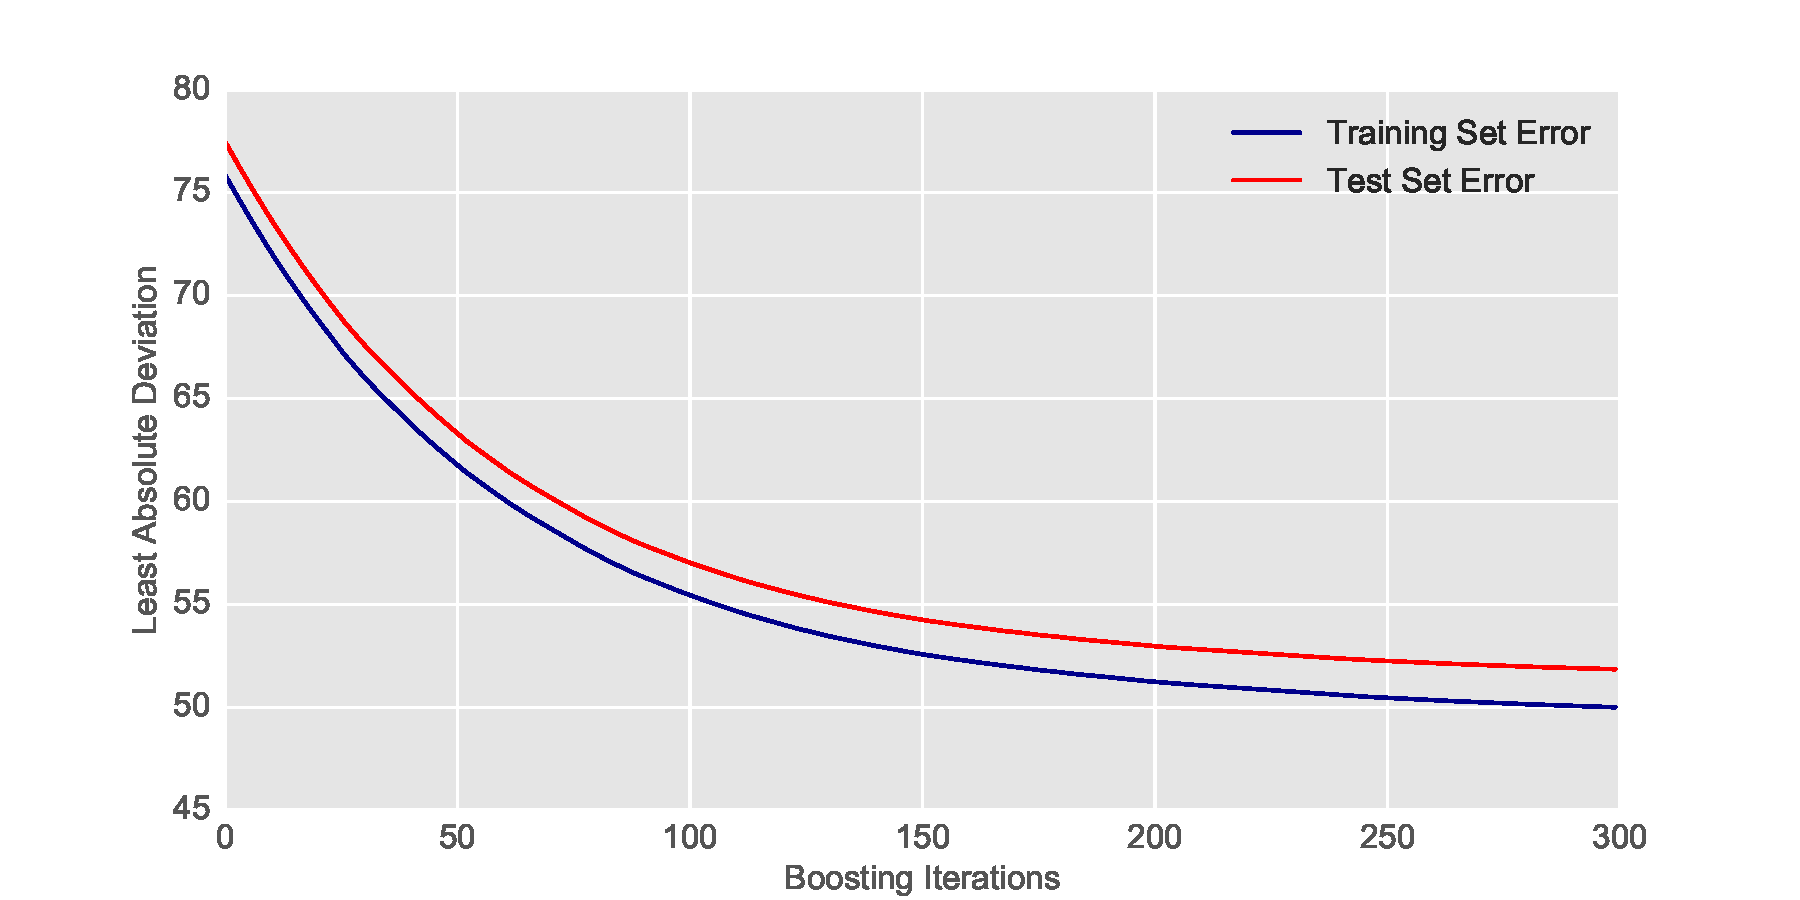
\includegraphics[width=\linewidth]{images/gradient_boosting_regressor_price}
%		\caption{Gradient Boosting Regressor - Error values affected by each round of boosting}
%		\label{fig:gradientboostingregressorprice}
%\end{figure}

%We can observe in Figure~\ref{fig:gradientboostingregressorprice} that the graph begins to converge between 150 and 200 iterations, but is still benefiting from more iterations, so we could increase the iterations to increase the results. 

After, we calculate the feature importances to see which features were most influential in predicting the listing price, Figure~\ref{fig:featureimportanc_gridSearchCVprice}. This show a relative scoring of how important each feature is relative to the feature with the most importance.

\begin{figure}[!htpb]
	\centering
	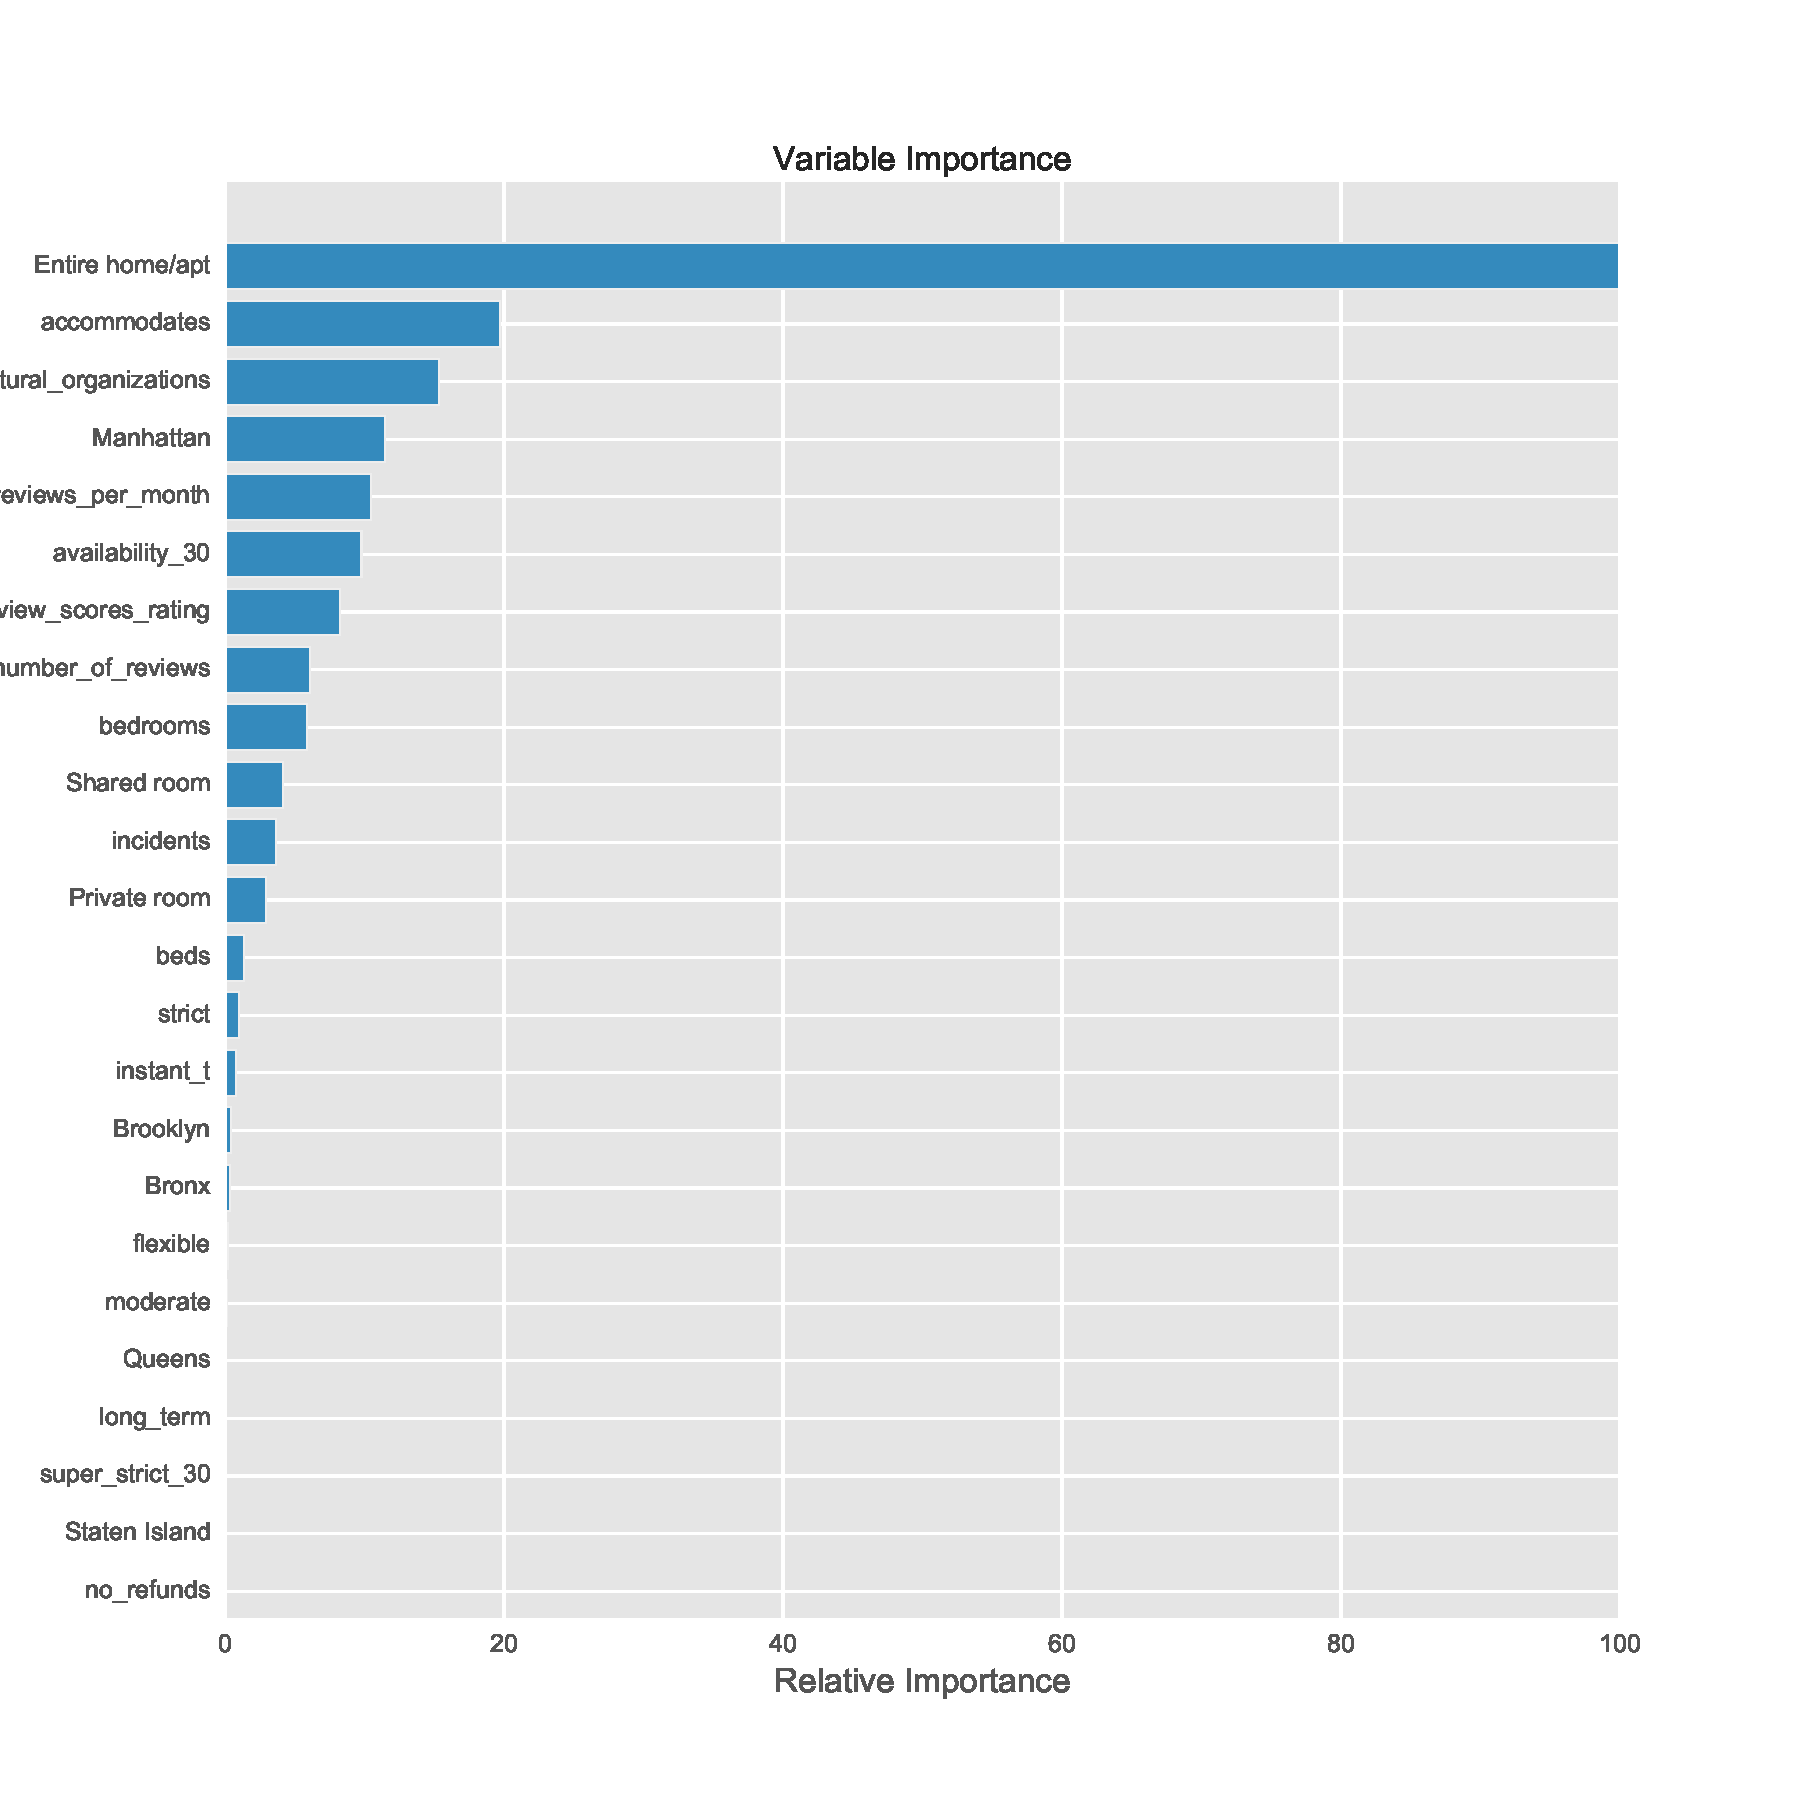
\includegraphics[width=\linewidth]{images/feature_importance_gridSearchCV_price}
	\caption{Gradient Boosting Regressor - Feature Importance}
	\label{fig:featureimportanc_gridSearchCVprice}
\end{figure}

Clearly some of the variables have more influence than others, and the most influential feature is the ``Entire home/apt'' attribute; this indicates whether or not the unit is shared with other people, and has the most effect in setting the price. This feature is followed by accommodates, cultural organizations and Manhattan district, and the feature incidents was not so influent. In this sense, we can conclude that the local is not so influent in to predict the price, but the room type.

\section{Problems found}
\label{sec:problemsfound}

We identified some points that can be problems found during the work: (i) The listings data set had problem to read it and a workaround was done using R language; (ii) Organizing the data to create a possible research question and answer it; and (iii) How to use machine learning to show something that could not be answered, i. e., using charts, maps or display the raw data in the DataFrame provided by Apache Spark.

\section{Concluding Remarks}
\label{sec:conclusion}

This work introduces an analysis trying to discovery if the cultural organizations and incidents influence on listing price. The ideia is to check the collinearity the features, try to predict the price using regression models, and to check the level importance of the features chose. 

We implemented and evaluated the New York City in relation the Airbnb listings. The results shows that where it has more cultural organization it has more incidents probability. Besides, the cultural organization was the third feature more influent in to predict the price. Using Gradient Boosting Regression we were able to fit a model that obtained a Median Absolute Error of \$23.91 for all listing data. 

For a practical predictor to be used in practice, future work will need to be done to further explore and build more suitable models. Predicting a significantly skewed right response variable, price, yields a set of challenges that need to be addressed rather than predicting a specific price. Future works could consider population density, property price, and an analysis by neighborhood.

\balance
\bibliographystyle{ACM-Reference-Format}
\bibliography{references} 

\end{document}